%\author{Олег Смирнов}

\documentclass[a4paper, 12pt]{article}

\usepackage[a4paper,hmargin=2.5cm,vmargin=2.5cm]{geometry}

\usepackage{amsfonts, amsmath, amssymb, amsthm, array, hhline, amscd, mathtools}
\usepackage{graphicx, wrapfig}
\usepackage{float}
\usepackage{upgreek}
\usepackage{enumerate}

\usepackage{color}

\usepackage[T1, T2A]{fontenc}
\usepackage[utf8]{inputenc}

%\usepackage[russian]{babel}

\graphicspath{{media/}}
\DeclareGraphicsExtensions{.pdf,.png,.jpg}

\newcommand{\bigs}{\vspace*{\bigskipamount}}

\usepackage{indentfirst}

\let\oldref\ref
\renewcommand{\ref}[1]{(\oldref{#1})}

\theoremstyle{definition}
\newtheorem*{definition}{Definition}

\theoremstyle{definition}
\newtheorem*{designation}{Designation}

\theoremstyle{proposition}
\newtheorem*{proposition}{Proposition}

\theoremstyle{lemma}
\newtheorem*{lemma}{Lemma}


\newcommand{\M}{\mathcal{M}}
\renewcommand{\l}{\lambda}
\newcommand{\m}{\mu}
\newcommand{\g}{\upgamma}
\renewcommand{\d}{\delta}
\newcommand{\D}{\Delta}
\newcommand{\T}{\Theta}


\newcommand{\Ts}[5][,]{%
	\begin{equation*}
		\T_{\g'} = \T_{#2},\;
		\T_{\g''} = \T_{#3},\;
		\T_{\d'} = \T_{#4},\;
		\T_{\d''} = \T_{#5}{#1}
	\end{equation*}%
}

\newcommand{\Tspairs}[3][,]{
	\begin{equation*}
		\T_{\g'} = \T_{\d'} = \T_{#2},\;
		\T_{\g''} = \T_{\d''} = \T_{#3}{#1}
	\end{equation*}
}

\newcommand{\uu}[2]{
	\dfrac{1 + p \T_{#1}}{1 + p \T_{#2}}\,
}

\newcommand{\up}[2]{
	\dfrac{1 + p \T_{#1}}{1 + p' \T_{#2}}\,
}

\newcommand{\pu}[2]{
	\dfrac{1 + p' \T_{#1}}{1 + p \T_{#2}}\,
}

\newcommand{\pp}[2]{
	\dfrac{1 + p' \T_{#1}}{1 + p' \T_{#2}}\,
}

\newcommand{\nn}[2]{
	\dfrac{1 + {#1}}{1 + {#2}}\,
}

\newcommand{\pic}[2][1]{%
	\begin{figure}[H]
		\centering
		\includegraphics[width=#1\textwidth]{#2}
	\end{figure}
}


\begin{document}
	
\section{Introductory notation}

\subsection{Markov and Lagrange values}

Symbol $\M$ denotes double-infinite sequences from $\mathbb{N}^\mathbb{Z}$:
\begin{equation*}
	\M = ...a_{-2}a_{-1}a_0a_1a_2...
\end{equation*}

I will use $\l(\M)$, $\m(\M)$ and $f(\M)$ for Lagrange, Markov values and height function.

Symbols $\g$ and $\d$ denote the lhs and rhs of sequence $\M$:
\begin{gather*}
	\g(\M) = [0; a_{-1}, a_{-2}, ...], \\
	\d(\M) = [0; a_1, a_2, ...], \\
	f(\M) = a_0 + \g(\M) + \d(\M).
\end{gather*}

At last, symbols $M$ and $L$ denote the Markov and Lagrange spectra.


\subsection{Centered sequences}

\begin{definition}
	A sequence $\M$ is called \textbf{centered}, if
	\begin{equation}\label{sup_in_0}
		\mu(\M) = f(\M).
	\end{equation}
\end{definition}

\begin{proposition}
	Markov spectrum can be defined with only centered sequences:
	\begin{equation*}
		\{ \m(\M) \mid \M \in \mathbb{N}^\mathbb{Z} \} =
		M =
		\{ \m(\M) \mid \M \text{ is centered } \}.
	\end{equation*}
\end{proposition}

%From now on we will only consider sequences satisfying \ref{centered}.
%and it will be omitted from here to the end of the book.


\subsection{Rectangle}

\begin{designation}
	Denote by
	\begin{equation*}%\label{rectangle}
		\left\{ a_{i_1}, a_{i_1 + 1}, ..., a_{i_2} \right\}
		\;(i_1 \leqslant 0 \leqslant i_2)
	\end{equation*}
	the set of double-infinite sequences $\M$
	with fixed terms $a_{i_1}, a_{i_1 + 1}, ..., a_{i_2}$
	on the corresponding positions.
	
	Terms $a_s$ for $s < i_1$ and $s > i_2$ are arbitrary integers,
	chosen such that $\M$ is centered and, maybe, satisfies some conditions.
\end{designation}

Segments $\D_1$, $\D_2$ and $\D$
are defined by the following equations:
\begin{equation}\label{deltas}
	\begin{array}{lclcl}
		\D_1 & = & \left[\, \D_1' \,;\, \D_1'' \, \right]
		& = & \left[\, \min\g( \M) \,;\,
		\max\g( \M) \, \right],
		\\
		\D_2 & = & \left[\, \D_2' \,;\, \D_2'' \, \right]
		& = & \left[\, \min\d( \M) \,;\,
		\max\d(\M) \, \right],
		\\
		\D & = & \left[\, \D' \,;\, \D'' \, \right]
		& = & a_0 + \D_1 + \D_2,
	\end{array}
\end{equation}
where $\M$ belongs to the rectangle.

\begin{definition}
	\textbf{Rectangle} is the segment $\D$ with the set of sequences, defining it.
\end{definition}

\begin{definition}
	Call a rectangle $\D$ \textbf{horizontal}, if
	\begin{equation}
		\label{d1>d2}
		|\D_1| \geqslant |\D_2|.
	\end{equation}
\end{definition}

Clearly, we can always obtain a horizontal rectangle out of the vertical one,
as we can reindex the sequence in the opposite direction.

\subsection{Resection}

\begin{definition}
	Call \textbf{resection} of a segment $A = [a; b]$
	a process of removing subsegment $A_{12} = [a_1; b_1]$,
	leaving two segments $A_1 \sqcup A_2 = [a; a_1] \sqcup [b_1; b]$.
\end{definition}

%We will introduce an infinite sequence of resections
%(at first segment $A$ is resected, then resections are performed at $A_1$ and $A_2$, and so on)
%which will produce Cantor set $\mathcal{L}(A)$.

\begin{definition}
	Call subsegment $A_{12} \subset A$ \textbf{normal}, if it is thicker than the two remaining subsegments:
	\begin{equation}
		\label{normal_resection}
		|A_{12}| \leqslant min\;\{|A_1|,\; |A_2|\}
	\end{equation}
\end{definition}

We call a resection \textbf{normal} if the resected subsegment is normal.

\begin{proposition}
	For any normal resection, having
	\begin{equation}
		\label{sum_is_present}
		A + A = (A_1 \sqcup A_2) + (A_1 \sqcup A_2).
	\end{equation}
\end{proposition}

%Clearly, if segment $A$ is transformed into Cantor set $\mathcal{L}(A)$ with only normal resections, then
%\begin{equation*}
%	A + A = \mathcal{L}(A) + \mathcal{L}(A).
%\end{equation*}

%\textit{We will \textbf{only} perform normal resections during the proof.}


\subsection{Subrectangle}
Consider a rectangle $\D$, set by the sequence center
\begin{equation*}
	\left\{ a_{i_1}, a_{i_1 + 1}, ..., a_{i_2} \right\}.
\end{equation*}

We will use a \textbf{shorter notation} for subrectangles, produced by setting integers
$a_i$ for $i < i_1$ or $i > i_2$:
\begin{equation*}
	\left\{ b_\ell...b_1,\; c_1...c_r\right\} \coloneqq
	\left\{ b_\ell...b_1 a_{i_1} ... a_{i_2} c_1...c_r\right\}.
\end{equation*}

For example:
\begin{equation}\tag{ex.1}\label{subrectangle_ex1}
	\left\{213, 3\right\} := \left\{ 213 a_{i_1} ... a_{i_2} 3\right\},
\end{equation}
\begin{equation}\tag{ex.2}\label{subrectangle_ex2}
	\left\{2, 0\right\} := \left\{ 2 a_{i_1} ... a_{i_2}  \right\}.
\end{equation}

We will also shorter the notation \ref{deltas}: lhs and rhs are $\D_1(312)$ and $\D_2(3)$ for subrectangle \ref{subrectangle_ex1} and $\D_1(2)$ and $a_2$ for \ref{subrectangle_ex2}.


\subsection{Geometrical interpretation}

Markov spectrum $M$ is the projection of some subset $\mathcal{S} \subset C_4 \times C_4$ onto the diagonal.

In these terms, \textbf{rectangle} is a rectangle and \textbf{subrectangles} are its subrectangles.

We will consider a family of rectangles whose projections cover the beginning of Hall's Ray.

Then we will present the algorithm to split rectangle into subrectangles so that their projections cover the projections of initial rectangle.

The more <<squarish>> the rectangle, the easier the step.

That's why we will bound the aspect ratio of rectangles (see \textbf{good} rectangle).

Formulas to evaluate aspect ratio are given in section \oldref{section_calculations}.

\newpage
\section{Calculations}
\label{section_calculations}

\subsection{Length of $\D_1$ or $\D_2$}
\label{useful_equality}

Let's fix some terms of continued fraction $[0; q_1, q_2, q_3, ..., q_n]$.

We will often need to measure difference
\begin{equation*}
	[0; q_1, q_2, q_3, ..., q_n, \dfrac{1}{\T_R}] - 
	[0; q_1, q_2, q_3, ..., q_n, \dfrac{1}{\T_L}],
\end{equation*}

where $\T$'s are some continuations of the continued fraction.

They generally look like $\T = [0;12\overline{13}]$ or something\footnote{%
	Here, as always in this book, $\overset{k}{\overline{abc}}$
	means $k$-times repetition of $abc$,
	and $\overline{abc}$ means infinite repetition.}.
We will set $\T$'s explicitly.

For the general proof, $\T$'s will be taken from table \oldref{table_theta}.

\begin{designation}
	For given continuation $\T_i$ denote by $\varepsilon_i$ resulting continued fraction:
	\begin{equation}\tag{3.4}\label{epsilon_rule}
		\varepsilon_i = [0; q_1, q_2, ..., q_n, \frac{1}{\T_i}].
	\end{equation}
\end{designation}

Then the following equality takes place:

\begin{equation}\tag{3.5}\label{varepsilons_difference}
	| \varepsilon_i - \varepsilon_j | = 
	\dfrac{| \T_i - \T_j |}
	{Q_n^2 \left(1 + pQ_i\right) \left(1 + pQ_j\right)},
\end{equation}

where

\begin{equation*}
	p = \dfrac{Q_{n-1}}{Q_n}.
\end{equation*}

\subsection{Rectangle aspect ratio}

Consider some fixed center of rectangle $\{a_{i_1} ... a_{i_2}\}$.

We will often extend it from the left (right) using some continuations
$\T_{\g_1}, \T_{\g_2}\; (\T_{\d_1}, \T_{\d_2})$.

These values produce $\g_1$, $\g_2$ ($\d_1$, $\d_2$)
using \ref{epsilon_rule}.

In other words, finite continued fractions
$[0; a_{-1}, a_{-2}, ..., a_{i_1}] = \dfrac{P_{i_1}}{Q_{i_1}}$
$\left([0; a_{1}, a_{2}, ..., a_{i_2}] = \dfrac{P_{i_2}}{Q_{i_2}}\right)$
are convergents for $\g_1$, $\g_2$ ($\d_1$, $\d_2$).

Then

\begin{equation}%\tag{5.6}\label{one_more_equation}
	\left| \dfrac{\g_1 - \g_2}{\d_1 - \d_2} \right|
	=
	\dfrac{1}{q}
	\left| \dfrac{\T_{\g_1} - \T_{\g_2}}
	{\T_{\d_1} - \T_{\d_2}} \right|
	\dfrac{1 + p' \T_{\d_1}}{1 + p \T_{\g_1}}\,
	\dfrac{1 + p' \T_{\d_2}}{1 + p \T_{\g_2}}
	\approx
	\dfrac{1}{q}
	\left| \dfrac{\T_{\g_1} - \T_{\g_2}}
	{\T_{\d_1} - \T_{\d_2}} \right|,
\end{equation}
where
\begin{equation*}
	p = \dfrac{Q_{i_1 + 1}}{Q_{i_1}},\;\;
	p' = \dfrac{Q_{i_2 - 1}}{Q_{i_2}},\;\;
	q = \dfrac{Q_{i_1}^2}{Q_{i_2}^2}.
\end{equation*}

\section{Rectangle boundaries}
\label{section_boundaries}

\subsection{Nonformal}

Let $\{\d_n\}$ be set of fractions
$\d_n = [0; q_1, q_2, ..., q_n, ...]$ with $n$ fixed terms.
We will suppose that $n$ is even (for odd $n$ the bounds are swapped).

At first, determine the smallest of fractions $\d_n$.

We will consider 2 cases: $S$
(\underline{S}hortened) and $N$ (\underline{N}ormal):

\begin{equation}
	\label{left_shortened_normal}
	\begin{array}{ll}
		S. & q_{n-1} = 3, q_n = 1. \\
		N. & \text{Otherwise.}
	\end{array}
\end{equation}

The lower bound $\d_n'$ for segment, containing $\d_n$, is defined by:
\begin{equation}
	\begin{array}{ll}
		S. & \hspace*{15pt} \d_n' = [0; q_1, ..., q_n, 213\overline{12}]. \\
		N. & \hspace*{15pt} \d_n' = [0; q_1, ..., q_n, 3\overline{12}].
	\end{array}
\end{equation}

To set the upper bound $\d_n''$ -- biggest of $\d_n$, consider 2 other cases:
\begin{equation}
	\begin{array}{ll}
		S. & \hspace*{15pt} q_{n} = 3.\\
		N. & \hspace*{15pt} q_{n} \ne 3.
	\end{array}
\end{equation}

Then

\begin{equation}
	\begin{array}{ll}
		S. & \hspace*{15pt} \d_n'' = [0; q_1, ..., q_n, 1213\overline{12}]. \\
		N. & \hspace*{15pt} \d_n'' = [0; q_1, ..., q_n, 13\overline{12}].
	\end{array}
\end{equation}

These bounds will allow us to construct sequences $\M$,
for which combination $(31313)$ is forbidden and, therefore,
the following condition takes place:
\begin{equation}
	f_i(\M) \leqslant \lambda(\overline{31312}) \approx 4,5241, \;
	i \ne 0,
\end{equation}
which will ensure \ref{centered}.

\subsection{Formal}

Let's now turn to concrete definitions and bounds. Remind that \ref{horizontal}.

Suppose $i_1 = i_2 \pmod 2$, $i_1$ is even.

\subsubsection{Bounds for $\D'$}

\begin{enumerate}[I.]
	\item Suppose both $\{\g_0(\M)\}$ and $\{\d_0(\M)\}$
	don't meet condition \ref{left_shortened_condition} but meet \ref{left_normal}.
	We will denote such situation by $H-H-H$
	(segment $\D_1$ is left-normal, $\D_2$ is left-normal, rectangle $\D$ is normal).
	
	In this case define $\D'$ by equation
	\begin{equation}\tag{11.9}
		\D' = \lambda(\overline{21}3a_{i_1}... a_{i_2}3\overline{12}).
	\end{equation}
	
	\item[IIa.] Sets $\{\g_0(\M)\}$ and $\{\d_0(\M)\}$
	don't meet condition \ref{left_shortened_condition} but meet \ref{left_shortened}.
	This is case $H-H-Y$
	(segments $\D_1$ and $\D_2$ are left-normal, rectangle $\D$ is left-shortened).
	
	Then
	\begin{equation}\tag{11.10}\label{bound_l_hhy}
		\D' = \lambda(\overline{21}3a_{i_1}... a_{i_2}213\overline{12}).
	\end{equation}
	
	\item[IIb.] Set $\{\g_0(\M)\}$ doesn't meet \ref{left_shortened_condition},
	$\{\d_0(\M)\}$ does.
	No matter, what takes place, \ref{left_shortened} of \ref{left_normal}.
	It is case $H_Y$
	(segment $\D_1$ is left-normal, segment $\D_2$ left-shortened).
	Bound $\D_1$ is defined by \ref{bound_l_hhy}.
	
	\addtocounter{enumi}{1}
	\item Set $\{\g_0(\M)\}$ meets \ref{left_shortened_condition},
	$\{\d_0(\M)\}$ doesn't.
	In this ($Y-H$) case $\D'$ is defined by the following:
	\begin{equation}\tag{11.11}\label{bound_l_yh}
		\D' = \lambda(\overline{21}312a_{i_1}... a_{i_2}3\overline{12}).
	\end{equation}
	
	\item Both $\{\g_0(\M)\}$ and $\{\d_0(\M)\}$
	meet \ref{left_shortened_condition}.
	In this ($Y-Y$) case $\D'$ is defined by
	\begin{equation}\tag{11.12}
		\D' = \lambda(\overline{21}312a_{i_1}... a_{i_2}213\overline{12}).
	\end{equation}
\end{enumerate}

\begin{figure}[p]
	\centering
	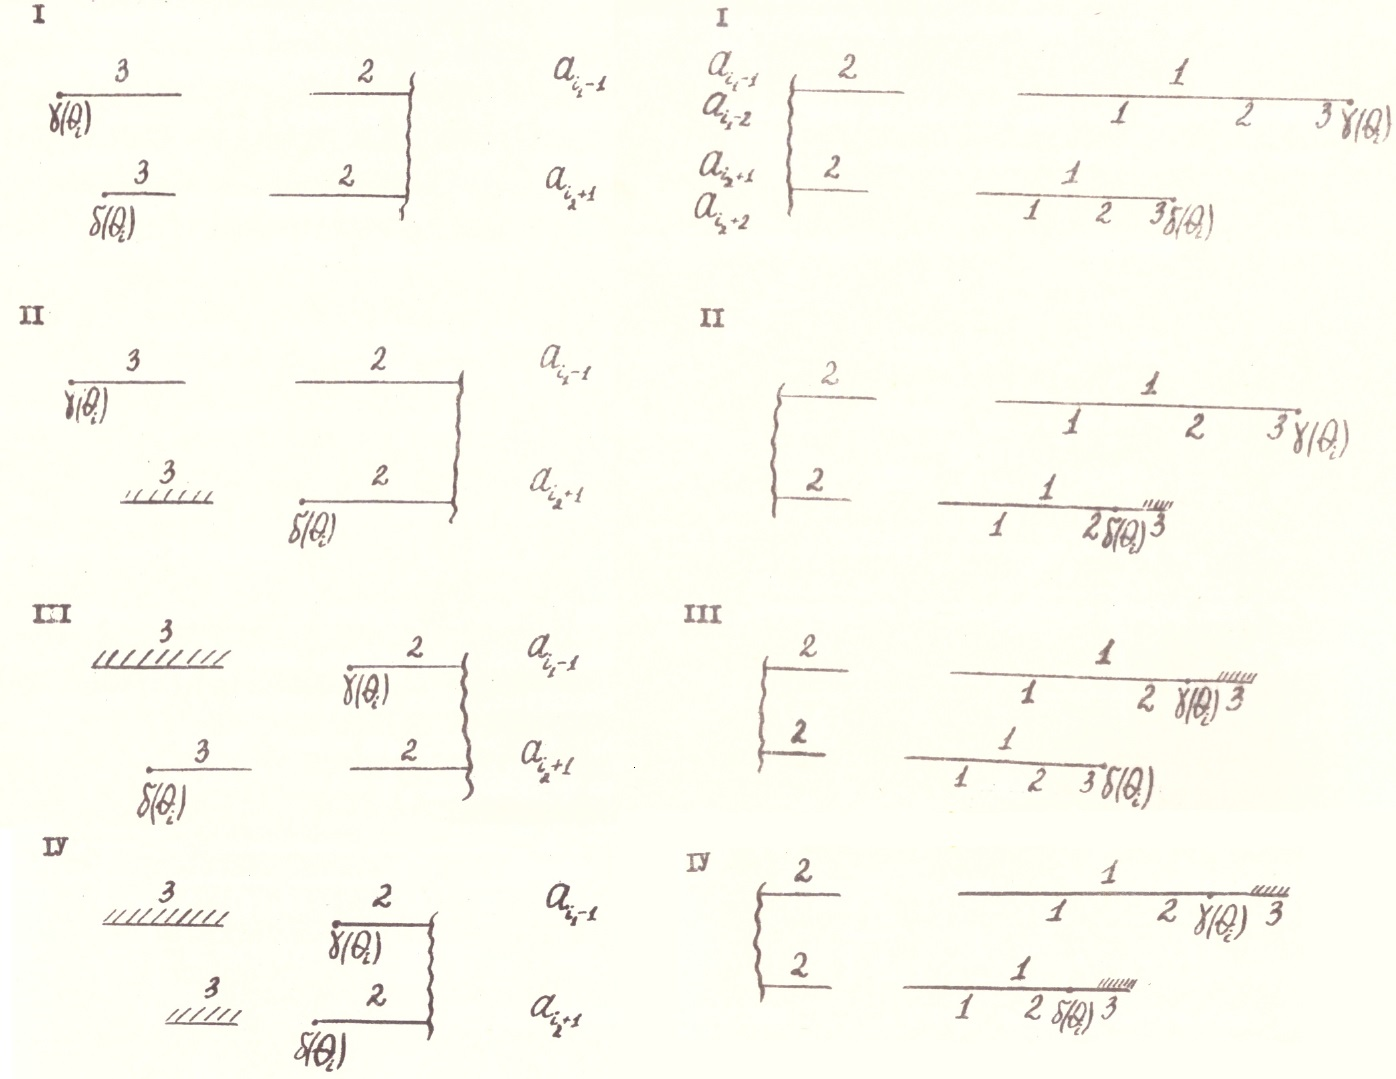
\includegraphics[width=0.9\textwidth]{pic1}
	\caption{Bounds $\D'$ (left) and $\D''$ (right).}
	\label{pic1}
\end{figure}

Figure \ref{pic1} illustrates the bounds. On the picture:

$\D_1' = \g(\T_i)$, $i=3,30$,
$\D_2' = \d  (\T_i)$, $i=3,30$,
$\D' = \D_1' + \D_2'$.

Hatched areas correspond to values of $a_{i_1 - 1}$ or $a_{i_2 + 1}$ (equal 3),
which can not appear in concrete case.

\subsubsection{Bounds for $\D''$}
Now we will provide formulas for $\D''$:

\begin{equation}\tag{11.13}
	\D'' = \lambda(\overline{21}31a_{i_1}... a_{i_2}13\overline{12})
\end{equation}
\begin{equation}\tag{11.14}
	\D'' = \lambda(\overline{21}31a_{i_1}... a_{i_2}1213\overline{12})
\end{equation}
\begin{equation}\tag{11.15}
	\D'' = \lambda(\overline{21}3121a_{i_1}... a_{i_2}13\overline{12})
\end{equation}
\begin{equation}\tag{11.16}
	\D'' = \lambda(\overline{21}3121a_{i_1}... a_{i_2}1213\overline{12})
\end{equation}

Figure \ref{table1} regulates the choose of the formulas.

\begin{figure}[ht]
	\centering
	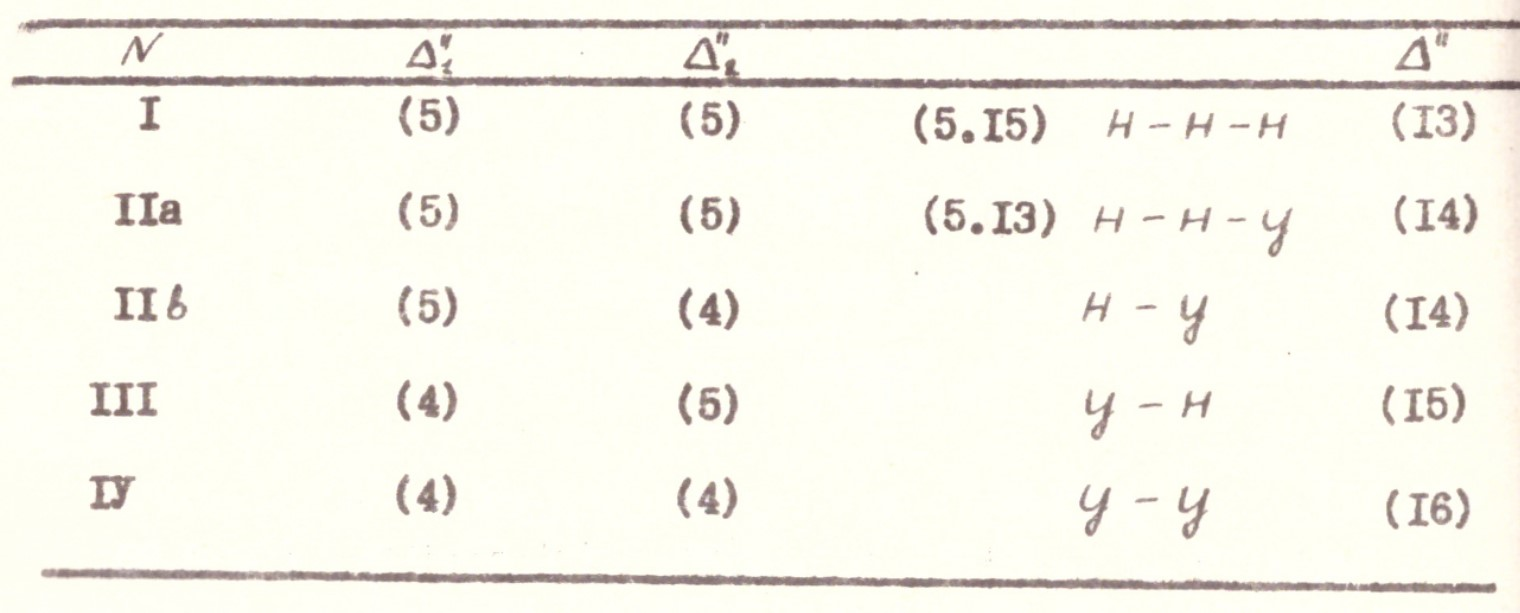
\includegraphics[width=0.8\textwidth]{table1}
	\caption{Rules for choose of $\D''$ in case $i_1 = i_2 \pmod 2$.}
	\label{table1}
\end{figure}

On the figure \ref{pic1}:
$\D_1'' = \g(\T_i)$, $i = 90, 94$,
$\D_2'' = \d  (\T_i)$, $i = 90, 94$,
$\D'' = \D_1'' + \D_2''$.
Hatched areas correspond to restricted value 3 of variables
$a_{i_1 - 2}$ or $a_{i_2 + 2}$.

\subsubsection{Case $i_1 \not\equiv i_2 \pmod 2$}

Now take case $i_1 \not\equiv i_2 \pmod 2$, $i_1$ is even. We will use rules from figure \ref{table2} to choose one of 4 formulas for $\D'$.

\begin{equation}\tag{11.17}
	I \hspace{15pt}
	\D' = \lambda(\overline{21}3a_{i_1}... a_{i_2}13\overline{12})
\end{equation}
\begin{equation}\tag{11.18}
	II \hspace{15pt}
	\D' = \lambda(\overline{21}3a_{i_1}... a_{i_2}1213\overline{12})
\end{equation}
\begin{equation}\tag{11.19}
	III \hspace{15pt}
	\D' = \lambda(\overline{21}312a_{i_1}... a_{i_2}13\overline{12})
\end{equation}
\begin{equation}\tag{11.20}
	IV \hspace{15pt}
	\D' = \lambda(\overline{21}312a_{i_1}... a_{i_2}1213\overline{12})
\end{equation}

\begin{figure}[ht]
	\centering
	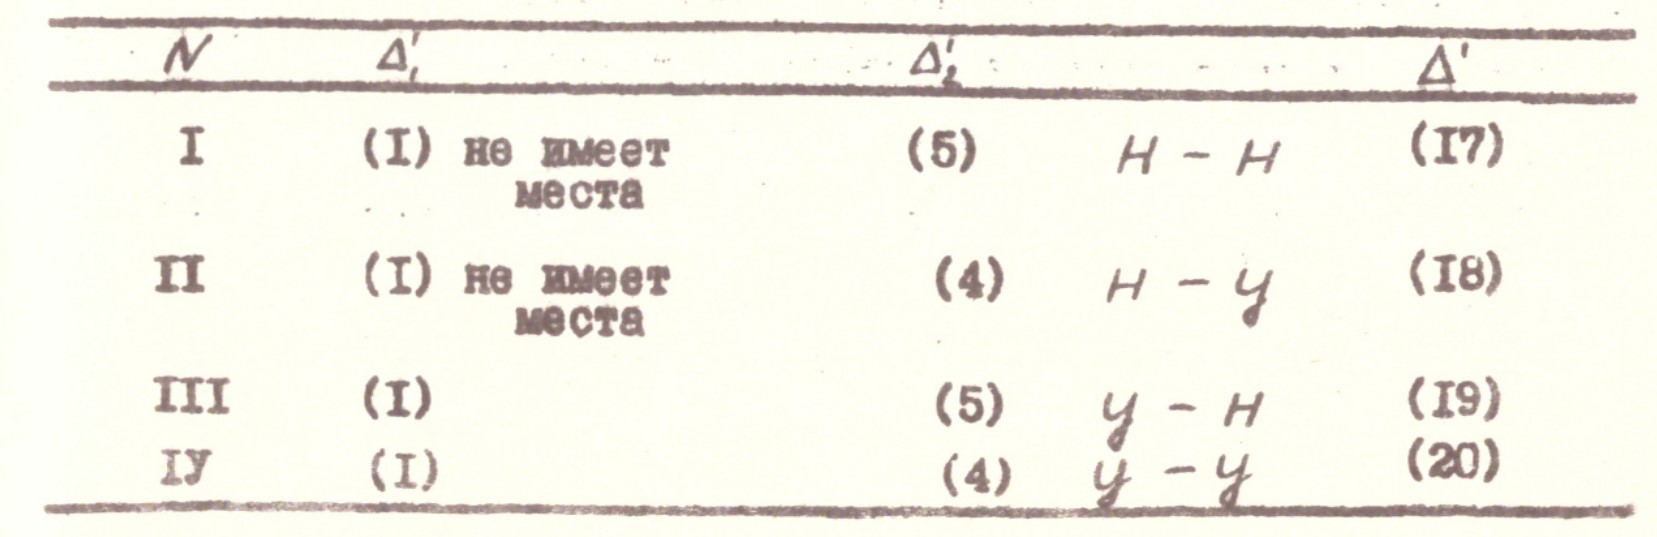
\includegraphics[width=0.8\textwidth]{table2}
	\caption{Rules for choose of $\D'$ in case $i_1 \ne i_2 \pmod 2$, $i_1$ is even.}
	\label{table2}
\end{figure}

To determine $\D''$ we will use rectangle
$$\{1, 0\}.$$
For this rectangle have $i_1 - 1 \equiv i_2 \pmod 2$, so we can use all the previous formulas to determine $\D''$.

\section{Good rectangle}
\label{section_good}

\subsection{Definition}

\begin{definition}
	Rectangle $\left\{ a_{i_1} ... a_{i_2} \right\}$ is \textbf{good},
	if subrectangles
	$\{2, 0\}$ and $\{1, 0\}$ intersect.
\end{definition}

For example, in case $i_1$ is even, that means

\begin{equation}\tag{6.3}\label{goodness}
	\{2, 0\}'' \geqslant \{1, 0\}'.
\end{equation}

Bounds of rectangles are determined by rules from section \ref{section_boundaries}.

If rectangle is not good (for example, \ref{goodness} doesn't take place), then
$$ ( \{2, 0\}'' ; \{1, 0\}' ) \not\subset
f \left\{ a_{i_1} ... a_{i_2} \right\}. $$
This is why goodness is necessary for the way we want to prove Freiman's constant.

\subsection{Sufficient conditions of goodness}

\subsubsection{Results}

Rectangle $\left\{ a_{i_1} ... a_{i_2} \right\}$ is good, if
\begin{equation}\label{goodness_condition}
	\dfrac{\D_1}{\D_2} <
	\left\{\begin{array}{ll}
		3.8, & i_1 \equiv i_2 \pmod 2,\\
		3.43, & i_1 \not\equiv i_2 \pmod 2.
	\end{array}\right.
\end{equation}

\subsubsection{Universal $2,9$ bound}

Now let's introduce some sufficient conditions for rectangle to be good.

%We will follow the same path as we did in \textsection 6.

Remind that we suppose $|\D_1| \geqslant |\D_2|$, which means

\begin{equation*}
	q
	\dfrac{1 + p \T_{1}}{1 + p' \T_{1}}
	\dfrac{1 + p \T_{95}}{1 + p' \T_{95}} \leqslant 1.
\end{equation*}

Let's introduce the following designations:
\begin{equation*}
	\g = [0; a_{-1}, ..., a_{i_1}, \frac{1}{\T_\g}],
\end{equation*}
\begin{equation*}
	\d = [0; a_{1}, ..., a_{i_2}, \frac{1}{\T_\d}],
\end{equation*}

where $\T$'s are some $\T$'s from Figure \ref{table_theta},
specified in each case separately.

\begin{figure}[p]
	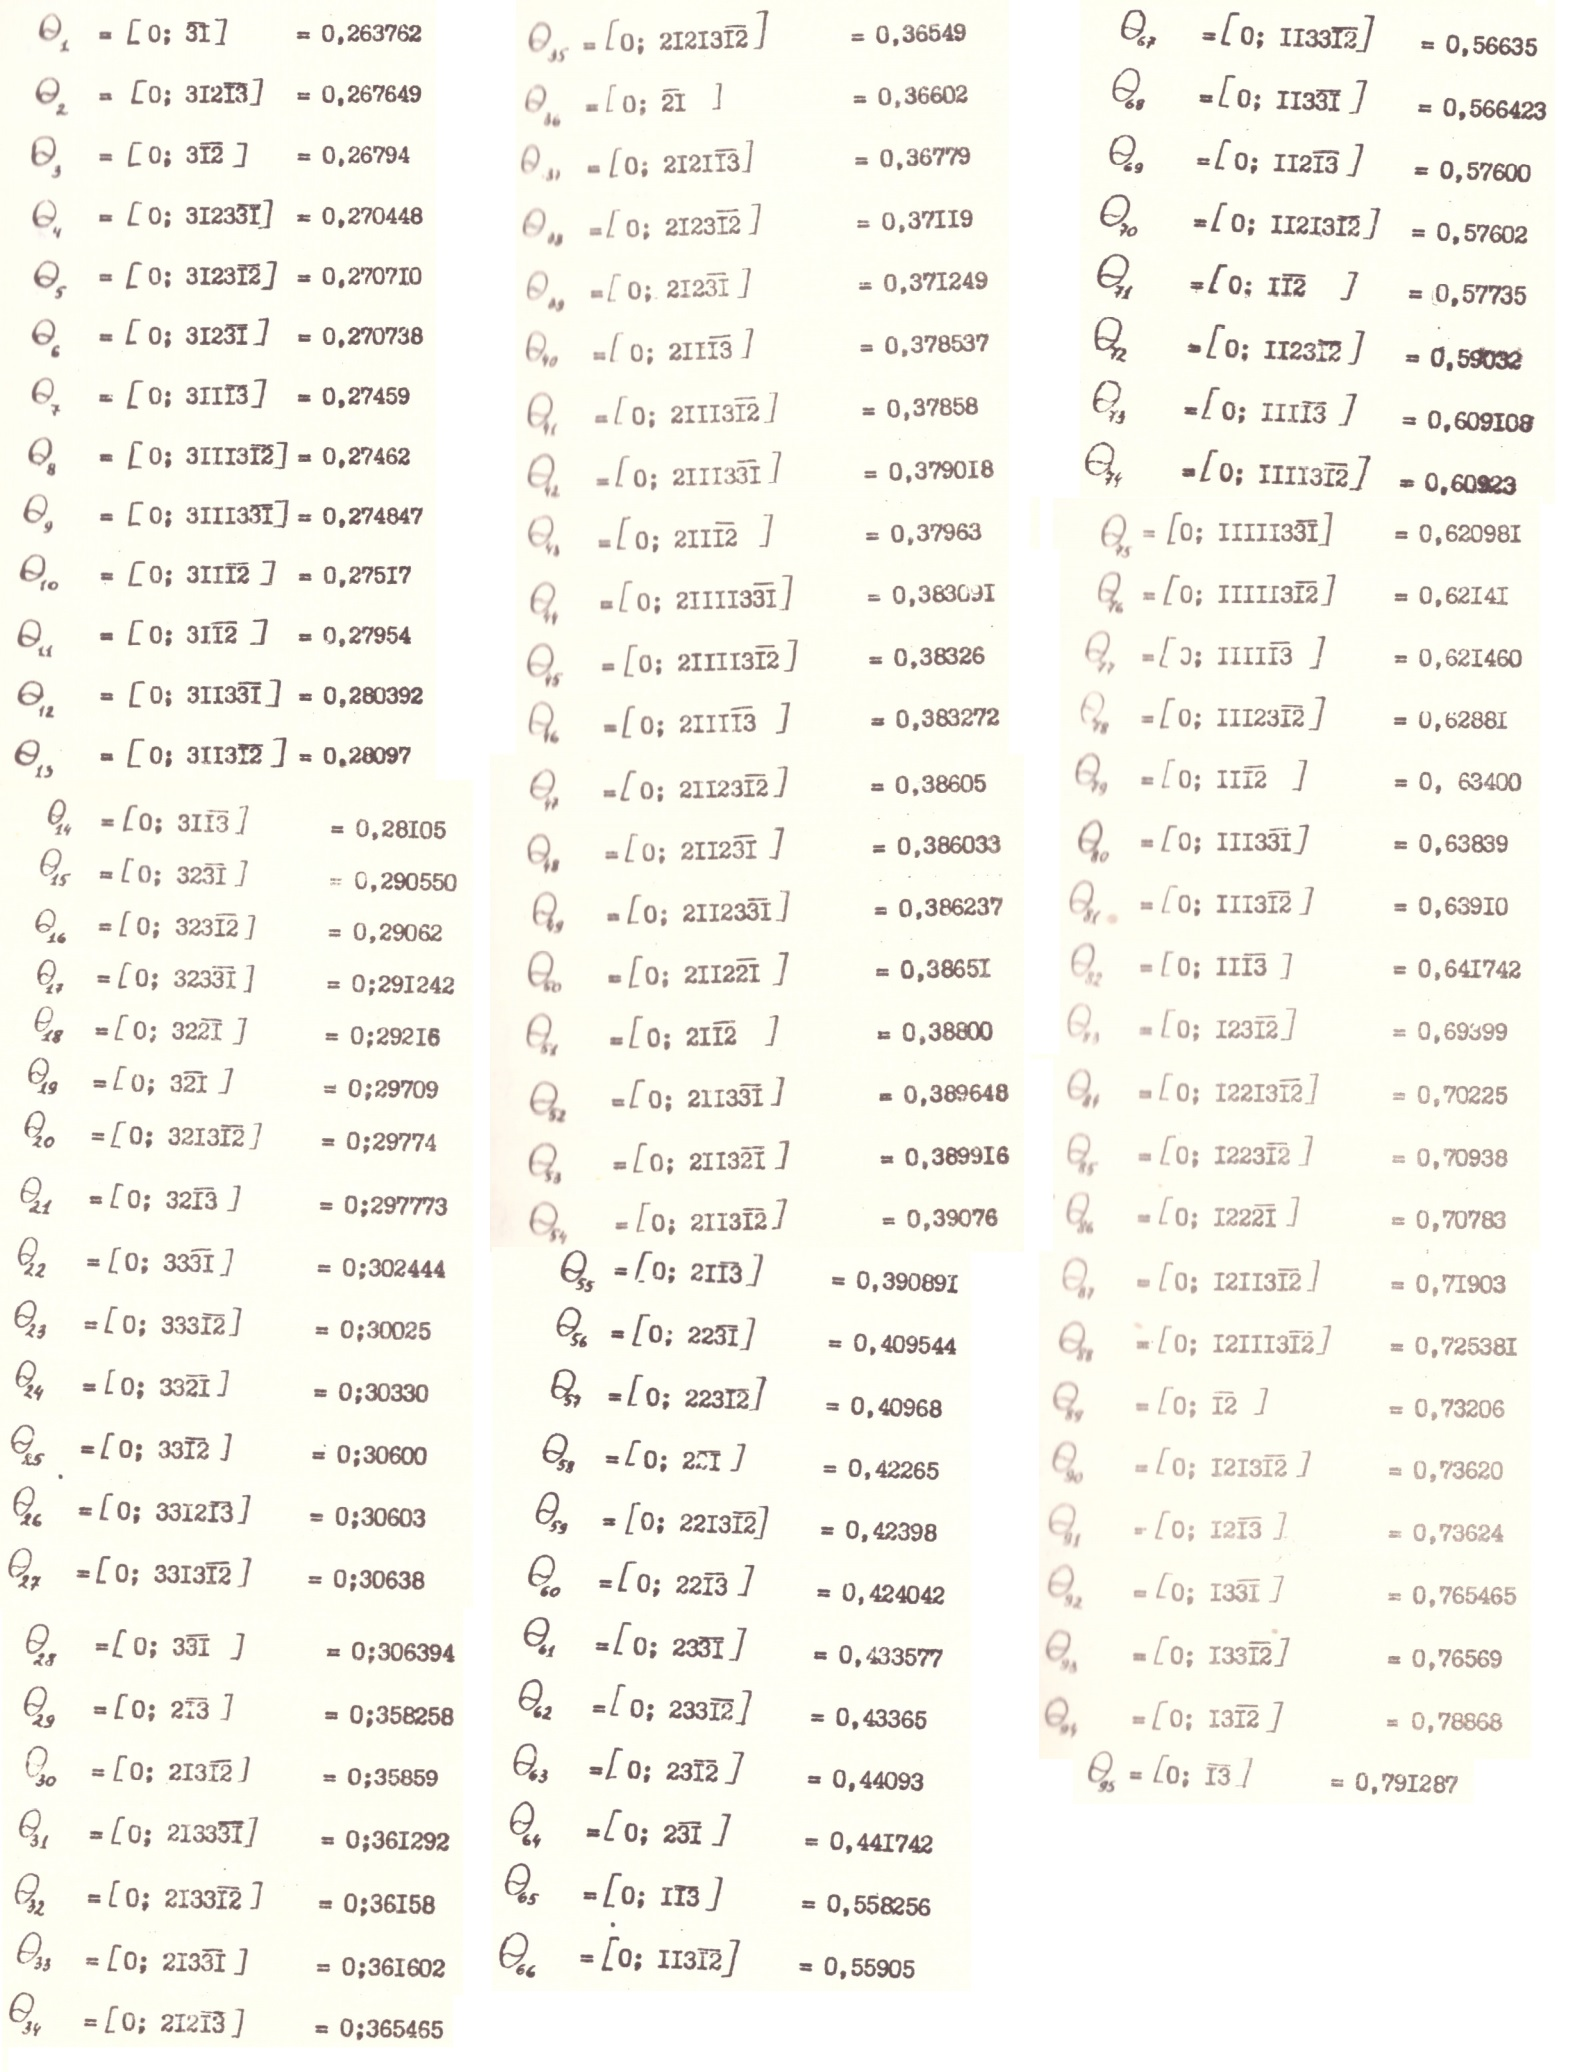
\includegraphics[width=\textwidth]{table_theta}
	\caption{Table of $\T$'s.}
	\label{table_theta}
\end{figure}

If rectangle is good, then \ref{goodness_in_deltas} should take place:

\begin{equation}\tag{12.1}\label{goodness_in_deltas}
	\g' - \g'' < |\d' - \d''|,
\end{equation}

where
$\T_{\g'} = \T_{66}$,
$\T_{\g''} = \T_{63}$,
$\T_{\d'} = \T_{90}$,
$\T_{\d''} = \T_{30}$.

{
	\itshape
	As I understand, theese thetas are supposed to be
	$\g' = \g_{\{1, 0\}}'$,
	$\g'' = \g_{\{2, 0\}}''$,
	and \ref{goodness_in_deltas} is just paraphrasing of \ref{goodness}
	in the «worst» case.
	As usual, Freiman gives no comments.
}

Inequality \ref{goodness_in_deltas} transforms into

\begin{equation}\tag{12.2}\label{12.2}
	0,313 <
	q
	\dfrac{1 + p \T_{63}}{1 + p' \T_{30}}
	\dfrac{1 + p \T_{66}}{1 + p' \T_{90}}.
\end{equation}

Suppose

\begin{equation}\tag{12.3}\label{goodness_condition_2,9}
	\dfrac{\D_1}{\D_2} < 2,9,
\end{equation}

which is equivalent to

\begin{equation}\tag{12.4}
	\dfrac{1}{q}
	\dfrac{1 + p' \T_{1}}{1 + p \T_{1}}
	\dfrac{1 + p' \T_{95}}{1 + p \T_{95}}
	<
	2,9.
\end{equation}

Then \ref{12.2} takes place. Indeed, it is so, if

\begin{equation*}
	\dfrac{1}{2,9}
	\dfrac{1 + p' \T_{1}}{1 + p \T_{1}}
	\dfrac{1 + p' \T_{95}}{1 + p \T_{95}}
	>
	0,313
	\dfrac{1 + p' \T_{30}}{1 + p \T_{63}}
	\dfrac{1 + p' \T_{90}}{1 + p \T_{66}}.
\end{equation*}

or, equivalent,

\begin{equation*}
	1,1
	>
	\dfrac{1 + p \T_{1}}{1 + p \T_{63}}
	\dfrac{1 + p \T_{95}}{1 + p \T_{66}}
	\dfrac{1 + p' \T_{30}}{1 + p' \T_{1}}
	\dfrac{1 + p' \T_{90}}{1 + p' \T_{95}},
\end{equation*}

Which is easily checked. \textit{Ha-ha}.

Condition \ref{goodness_condition_2,9} is sufficient for rectangle to be good,
no matter, are $i_1$ and $i_2$ equivalent $\pmod 2$ or not, take conditions
\ref{left_shortened_condition} and \ref{right_shortened_condition} place or not.

\subsubsection{Case $i_1 = i_2 \pmod 2$}

Now consider case $i_1 = i_2 \pmod 2$ (see picture):

\pic[0.5]{pic4}

We will suppose case $a_{i_2} = 1$, $a_{i_2 - 1} = 3$ doesn't take place.

We can substitute the folliwing $\g$'s and $\d$'s
into \ref{goodness_in_deltas}:

\Ts{66}{63}{90}{3}

and instead of \ref{12.2} we will get

\begin{equation}\tag{12.5}\label{12.5}
	0,253 < q
	\dfrac{1 + p \T_{63}}{1 + p' \T_{3}}
	\dfrac{1 + p \T_{66}}{1 + p' \T_{90}}.
\end{equation}

This choose of $\T_{\g'}$ and $\T_{\d''}$ is fine,
if the following inequality takes place:

\begin{equation}\tag{12.6}\label{goodness_condition_1,4}
	\d' - \d'' > 1,4 (\g' - \g''),
\end{equation}

where 
\begin{equation*}
	\T_{\g'} = \T_{68},\;
	\T_{\g''} = \T_{65},\;
	\T_{\d'} = \T_{28},\;
	\T_{\d''} = \T_{1},
\end{equation*}

so we can rewrite \ref{goodness_condition_1,4} as

\begin{equation}\tag{12.7}\label{12.7}
	0,253 < q
	\dfrac{1 + p \T_{65}}{1 + p' \T_{1}}
	\dfrac{1 + p \T_{68}}{1 + p' \T_{28}}.
\end{equation}

We can notice that \ref{12.7} follows from \ref{12.5}. Indeed, that follows from inequality

\begin{equation*}
	0,253
	\dfrac{1 + p' \T_{3}}{1 + p' \T_{63}}
	\dfrac{1 + p \T_{90}}{1 + p \T_{66}}
	>
	0,269
	\dfrac{1 + p' \T_{1}}{1 + p' \T_{65}}
	\dfrac{1 + p \T_{28}}{1 + p \T_{68}}
\end{equation*}

or inequality

\begin{equation*}
	\dfrac{1 + p \T_{65}}{1 + p \T_{63}}
	\dfrac{1 + p \T_{68}}{1 + p \T_{66}}
	\dfrac{1 + p' \T_{3}}{1 + p' \T_{1}}
	\dfrac{1 + p' \T_{90}}{1 + p' \T_{28}}
	>
	1,064.
\end{equation*}

{
	\itshape
	Here Freiman even omits comment «which is checked directly».
}

Overall, we proved that \ref{12.5} is enough for condition to be good.

Suppose

\begin{equation}\tag{12.8}\label{goodness_condition_3,8}
	\dfrac{\D_1}{\D_2} < 3,8
\end{equation}

or

\begin{equation*}
	\dfrac{1}{q}
	\dfrac{1 + p' \T_{1}}{1 + p \T_{1}}
	\dfrac{1 + p' \T_{95}}{1 + p \T_{95}}
	<
	3,8.
\end{equation*}

Then \ref{12.5} takes place. Indeed, it is so, if

\begin{equation*}
	\dfrac{1}{3,8}
	\dfrac{1 + p' \T_{1}}{1 + p' \T_{1}}
	\dfrac{1 + p \T_{95}}{1 + p \T_{95}}
	>
	0,253
	\dfrac{1 + p' \T_{3}}{1 + p' \T_{63}}
	\dfrac{1 + p \T_{90}}{1 + p \T_{66}}.
\end{equation*}

The last inequality is transformed into

\begin{equation*}
	1,04
	>
	\dfrac{1 + p' \T_{3}}{1 + p' \T_{1}}
	\dfrac{1 + p' \T_{90}}{1 + p' \T_{95}}
	\dfrac{1 + p \T_{1}}{1 + p \T_{63}}
	\dfrac{1 + p \T_{95}}{1 + p \T_{66}},
\end{equation*}

which is easy to check.

\subsubsection{Case $i_1 \ne i_2 \pmod 2$}

Now consider case $i_1 \ne i_2 \pmod 2$
and, again, case $a_{i_2} = 1$, $a_{i_2 - 1} = 3$
doesn't take place.
Suppose $i_1$ is even (see picture):

\pic[0.6]{pic5}

Taking
\begin{equation*}
	\T_{\g'} = \T_{66},\;
	\T_{\g''} = \T_{59},\;
	\T_{\d'} = \T_{3},\;
	\T_{\d''} = \T_{90},
\end{equation*}

rewrite \ref{goodness_in_deltas} as

\begin{equation}\tag{12.9}\label{12.9}
	0,2885
	<
	q
	\dfrac{1 + p \T_{59}}{1 + p' \T_{3}}
	\dfrac{1 + p \T_{66}}{1 + p' \T_{90}}.
\end{equation}

Suppose

\begin{equation}\tag{12.10}\label{goodness_condition_3,43}
	\dfrac{\D_1}{\D_2} < 3,43
\end{equation}

or

\begin{equation*}
	\dfrac{1}{q}
	\dfrac{1 + p' \T_{1}}{1 + p \T_{1}}
	\dfrac{1 + p' \T_{95}}{1 + p \T_{95}}
	<
	3,43.
\end{equation*}

Then \ref{12.9} takes place. Indeed, it is so, if

\begin{equation*}
	\dfrac{1}{3,43}
	\dfrac{1 + p' \T_{1}}{1 + p \T_{1}}
	\dfrac{1 + p' \T_{95}}{1 + p \T_{95}}
	>
	0,2885
	\dfrac{1 + p' \T_{3}}{1 + p \T_{59}}
	\dfrac{1 + p' \T_{90}}{1 + p \T_{66}}.
\end{equation*}

or

\begin{equation*}
	1,0105
	>
	\dfrac{1 + p' \T_{3}}{1 + p' \T_{1}}
	\dfrac{1 + p' \T_{90}}{1 + p' \T_{95}}
	\dfrac{1 + p \T_{1}}{1 + p \T_{59}}
	\dfrac{1 + p \T_{95}}{1 + p \T_{66}},
\end{equation*}

increasing the right part, obtain

\begin{equation*}
	1,0105
	>
	0,9896
	\dfrac
	{1 + p \cdot 1,0551 + p^2 \cdot 0,20875}
	{1 + p \cdot 0,983 + p^2 \cdot 0,237},
\end{equation*}

which is easily checked.

\newpage
\section{Freiman's constant. Initial set of rectangles}

All these rectangles satisfy \textit{\_here will be a complete list of conditions.\_}

At least all of them are good, in terms of section \oldref{section_good}.

%Their projections, in terms of section \oldref{section_boundaries}, cover the beginning of Hall's Ray.

\begin{figure}[H]
	\centering
	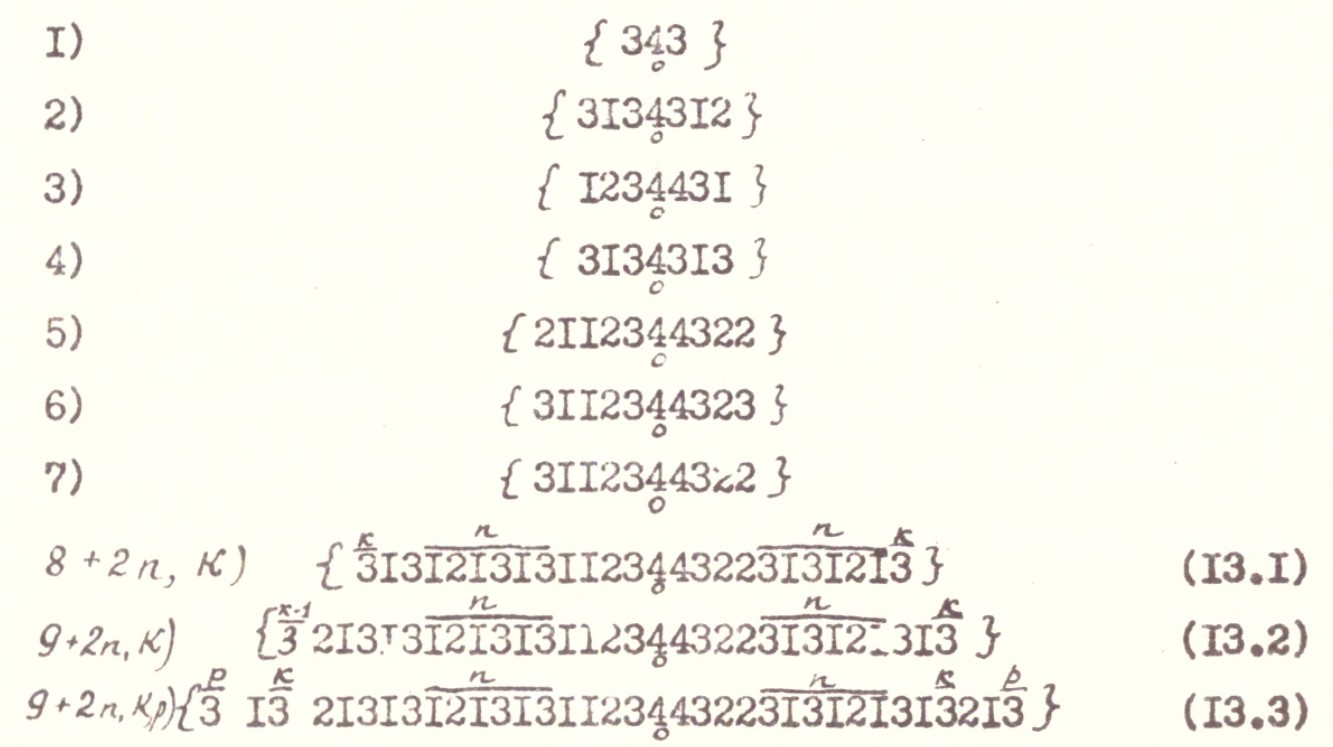
\includegraphics[width=0.8\textwidth]{initial_set}
	\caption{Freiman's constant. Initial set of rectangles.}
	\label{fc_init}
\end{figure}

%\begin{equation}\tag{}
%	1
%\end{equation}
%
%\begin{equation*}
%	1
%\end{equation*}

\newpage
\tableofcontents
	
\end{document} 

